\section{Auswertung}
\label{sec:Auswertung}

\begin{document}
\section{Auswertung}
\subsection{Bestimmung der Strömungsgeschwindigkeit als Funktion des Dopplerwinkels fur 5 verschiedene Flussgeschwindigkeiten}
In Tabelle \autoref{tab:1} befinden sich die gemessenen Frequenzverschiebungen und berechneten Strömungsgeschwindigkeiten für die Winkel $15$°, $30$° und $60$° zu der jeweiligen prozentualen Spannung der Zentrifugalpumpe für eine Röhre mit einem Außendurchmesser von 15 mm und einem Innendurchmesser von 10 mm.
\begin{table}[H]
  \centering
  \caption{Die gemessenen Frequenzverschiebungen und Strömungsgeschwindigkeiten für die Sondenwinkel 15°, 30° und 60° zu der jeweiligen prozentualen Spannung der Zentrifugalpumpe für eine Röhre mit einem Außendurchmesser von 15 mm und einem Innendurchmesser von 10 mm.}
  \begin{tabular}{l|l|l|l}
  $U$/$\%$ & $\alpha$/° & $\delta\nu$/Hz & $v$/$\textrm{ms}^{-1}$\\\hline
  45 & 15 & 61 & 0.159\\
     & 30 & 103 & 0.139\\
     & 60 & 171 & 0.133\\\hline
  50 & 15 & 85 & 0.222\\
     & 30 & 136 & 0.184\\
     & 60 & 218 & 0.170\\\hline
  60 & 15 & 106 & 0.276\\
     & 30 & 166 & 0.224\\
     & 60 & 280 & 0.218\\\hline
  65 & 15 & 133 & 0.347\\
     & 30 & 207 & 0.279\\
     & 60 & 333 & 0.260\\\hline
  70 & 15 & 186 & 0.485\\
     & 30 & 253 & 0.342\\
     & 60 & 448 & 0.349\\\hline
  \end{tabular}
  \label{tab:1}
\end{table}
Die Strömungsgeschwindigkeiten berechnen sich durch ....
Mit 
\begin{align*}
  \bar v&=\frac{1}{3}\sum\limits_{i=1}^{3} v_i\ \textrm{und}\\
  \Delta\bar v&=\sqrt{\frac{1}{6}\sum\limits_{i=1}^{3} (v_i - \bar x)^2}
\end{align*}
berechnen sich die mittleren Geschwindigkeiten und deren Fehler 
\begin{align*}
  \bar v_{45} \pm \Delta \bar v_{45}&=(0.144 \pm 0.01)\ \frac{\textrm{m}}{s},\\
  \bar v_{50} \pm \Delta \bar v_{50}&=(0.192 \pm 0.02)\ \frac{\textrm{m}}{s},\\
  \bar v_{60} \pm \Delta \bar v_{60}&=(0.239 \pm 0.02)\ \frac{\textrm{m}}{s},\\
  \bar v_{65} \pm \Delta \bar v_{65}&=(0.295 \pm 0.03)\ \frac{\textrm{m}}{s}\ \textrm{und}\\
  \bar v_{70} \pm \Delta \bar v_{70}&=(0.392 \pm 0.05)\ \frac{\textrm{m}}{s}
\end{align*}
für die Phantomflüssigkeit, angetrieben durch die prozentualen Spannungen der Zentrifugalpumpe.\\
Die Ergebnisse wurden in \autoref{fig:1} aufgetragen.
\begin{figure}[H]
  \centering
  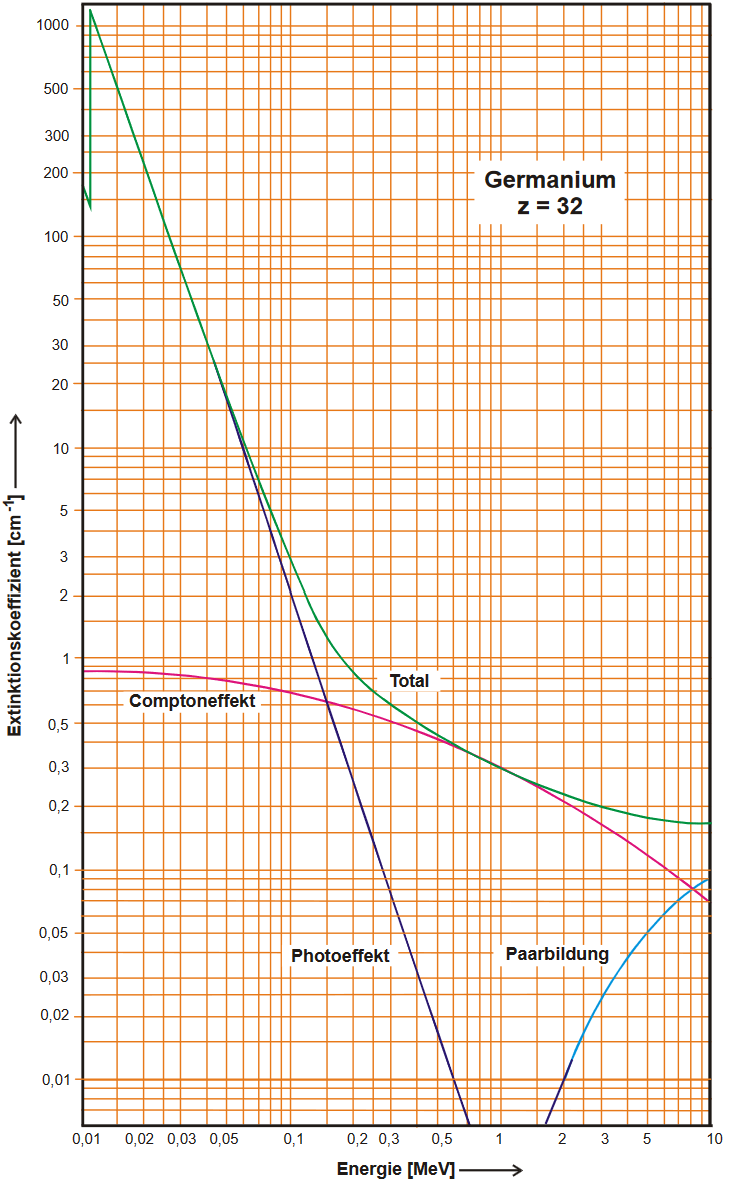
\includegraphics[width=12cm]{content/1}
  \caption{Die Strömungsgeschwindigkeit v aufgetragen gegen $\Delta\nu$/$\cos(\alpha)$.}
  \label{fig:1}
\end{figure}

\subsection{Bestimmung des Strömungsprofils der Doppler-Flüssigkeit an einem 3/8 Zoll Schlauch
mit einem Dopplerwinkel von 15°.}
Die gemessenen Geschwindigkeit und Streuintensitäten in Abhängigkeit der Meßtiefe bei einer Spannung von 45$\%$ und 70$\%$ für einen Sondenwinkel von 15° befinden sich in \autoref{tab.2}.
\begin{table}{H}
  \centering
  \caption{Die gemessenen Geschwindigkeit und Streuintensitäten in Abhängigkeit der Meßtiefe für einen Sondenwinkel von 15°.}
  \begin{tabular}{l|l|l|l|l}
  $x$/$\mu$s & $v_{45}$/$\textrm{ms}^{-1}$ & $I_{45}$/$10^3\cdot\frac{\textrm{V}^2}{\textrm{s}}$ & $v_{70}$/$\textrm{ms}^{-1}$ & $I_{70}$/$10^3\cdot\frac{\textrm{V}^2}{\textrm{s}}$\\\hline
  13.5 & - & - & 46.4 & 54\\
  14 & - & - & 42.2 & 43\\
  14.5 & - & - & 53 & 54\\
  15 & 23.9 & 70 & 58.3 & 76\\
  15.5 & 23.9 & 96 & 57 & 71\\
  16 & 22.5 & 115 & 50.4 & 86\\
  16.5 & 21.2 & 109 & 42.4 & 101\\
  17 & 18.6 & 83 & 35.8 & 99\\
  17.5 & 21.2 & 48 & 29.2 & 69\\
  18 & - & - & 29.2 & 36\\
  \end{tabular}
  \label{tab.2}
\end{table}
Die Geschwindigkeiten und Streuintensitäten für eine Spannung von 45$\%$ sind in \autoref{fig:2} gegen die Meßtiefe aufgetragen.
\begin{figure}[H]
  \centering
  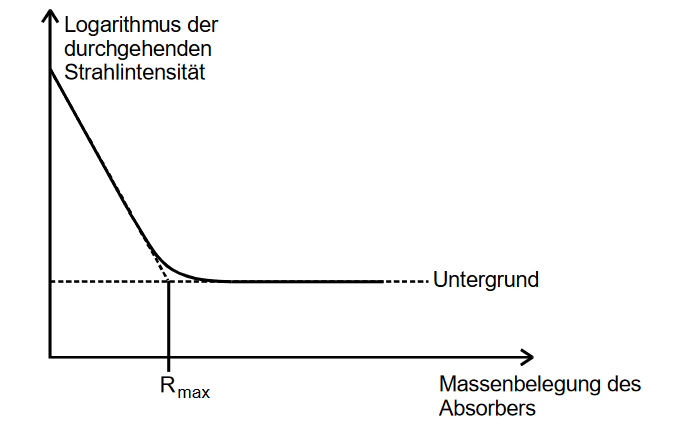
\includegraphics[width=12cm]{content/2}
  \caption{Die Geschwindigkeiten und Streuintensitäten aufgetragen gegen die Meßtiefe bei einer Spannung von 45$\%$.}
  \label{fig:2}
\end{figure}
Die Geschwindigkeiten und Streuintensitäten für eine Spannung von 75$\%$ sind in \autoref{fig:3} gegen die Meßtiefe aufgetragen.
\begin{figure}[H]
  \centering
  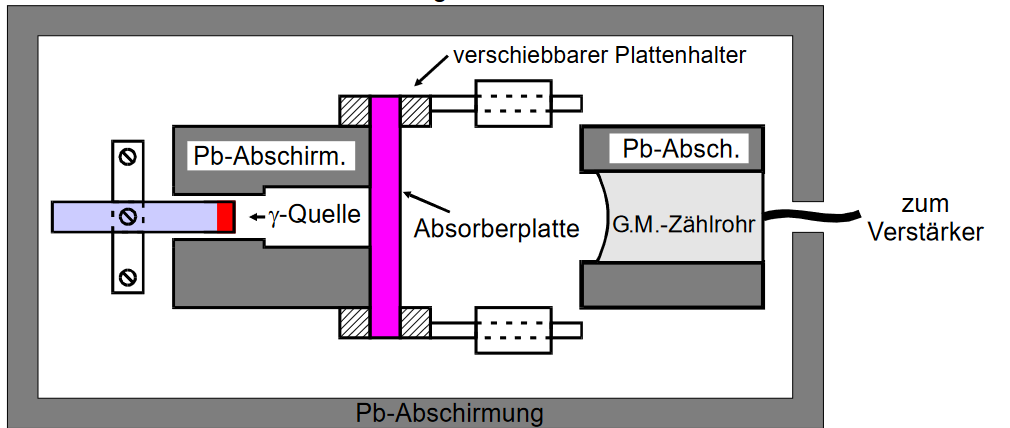
\includegraphics[width=12cm]{content/3}
  \caption{Die Geschwindigkeiten und Streuintensitäten aufgetragen gegen die Meßtiefe bei einer Spannung von 70$\%$.}
  \label{fig:3}
\end{figure}
